\documentclass[a4paper,twoside]{article}
\usepackage{graphicx}
\usepackage{calc}
\usepackage{amssymb}
\usepackage{amstext}
\usepackage{amsmath}
\usepackage{amsthm}
\usepackage{multicol}
\usepackage{pslatex}
\usepackage{apalike}
\usepackage{algorithm2e}
\usepackage[bottom]{footmisc}
\usepackage[T1]{fontenc}
\usepackage[utf8]{inputenc}
\usepackage{url}
\usepackage{SCITEPRESS}
\pdfinfo{/Title (Evidence-Grounded Agentic Dashboards: Numerical Validity, Answer Completeness, and Adaptive Presentation) /Author () /Subject (Anonymous author-review manuscript draft) /Keywords (Analytical agents; evidence provenance; longitudinal dashboards)}
% BEGIN GENERATED: numbers
\newcommand{\EnumVisible}{24}
\newcommand{\EnumSelected}{24}
\newcommand{\EnumAccepted}{24}
\newcommand{\AVisible}{21}
\newcommand{\ASelected}{18}
\newcommand{\AAccepted}{22}
\newcommand{\BVisible}{15}
\newcommand{\BSelected}{14}
\newcommand{\BAccepted}{24}
\newcommand{\CVisible}{15}
\newcommand{\CSelected}{11}
\newcommand{\CAccepted}{21}
% END GENERATED: numbers
\newcommand{\draftassist}{\footnote{Writing assistance: OpenAI Codex \cite{openaiCodex}; see Section~\ref{sec:disclosure}.}}
\begin{document}
\title{Evidence-Grounded Agentic Dashboards: Numerical Validity, Answer Completeness, and Adaptive Presentation}
\author{}
\keywords{Analytical Agents, Longitudinal Data, Evidence Provenance, Answer Completeness, Adaptive Dashboards.}
\abstract{Imagine a course adviser opening a dashboard and noticing a drop in a student's recorded activity. Has the student's usual pattern changed, does the comparison with classmates tell a different story, or are there too few observations to tell? We propose adaptive dashboards that organize the display around the question and available evidence. Personal timelines, peer comparisons, and clear indications of unavailable measurements are intended to help the operator interpret changes, examine alternative references, and recognize when evidence is insufficient. An agent selects analyses and answer content; deterministic tools calculate and validate quantities, while a later presentation layer arranges saved results. In 24 development cases from two Open University course offerings, three interfaces using Qwen2.5-14B-Instruct produced \AVisible, \BVisible, and \CVisible\ complete visible answers, compared with \EnumVisible\ for a rule based baseline. Correct numbers could still accompany a missing comparison or the wrong time window. Some judgments about equivalent answers remain unresolved; independent human review and held out evaluation are pending. The adaptive views demonstrate implemented presentation behavior, while their benefit to operators remains untested.}
\onecolumn\maketitle\normalsize\setcounter{footnote}{0}\vfill
\section{\uppercase{Introduction}}
\label{sec:intro}
\noindent A longitudinal question such as ``Has my activity changed, and am I different from my peers?'' contains several analytical choices. Activity must be operationalized; earlier and recent periods must be defined; peers must be identified; and eligibility and measurement availability must be checked. The same recorded value may be close to a contemporary course mean yet below that course's earlier mean. An absent recent value may indicate administrative ineligibility, while an eligible week with no recorded clicks is a recorded zero. A dashboard that obscures these distinctions can mislead even when its displayed arithmetic is correct.\draftassist

Retrieving a useful result, selecting the intended comparison, and displaying all requested answers are different accomplishments. A source-bound validator can verify a returned result without establishing that it answers the requested window. A compiler can supply essential context that the agent did not select. Evaluating only rendering success or agreement with source numbers would conflate these responsibilities.

We investigate this distinction in educational longitudinal dashboards. A model selects predefined analyses and answers; deterministic tools calculate quantities; validation checks evidence; and a compiler constructs claims and panels. A later presentation layer adapts saved content to personal change, reference comparisons, limited observations, and assessment records. This bounded application permits studying selection failures without delegating arithmetic or unrestricted frontend code to the model.

The empirical focus is a controlled comparison of three selection interfaces using the same checkpoint and analytical backend. A compact interface is compared with derived support/scope metadata and with additional explicit analytical identity. The hypothesis is that making feature, windows, reference, and peer-versus-personal meaning explicit reduces incompleteness. Deterministic enumeration answers the same task families.

Three research questions guide the study. First, does explicit answer identity improve complete valid visible answers under fixed tool and inference budgets? Second, how do conclusions change when completeness attributable to method selections is separated from completeness supplied by compiler context? Third, what do saved failures reveal about the distinction between retrieving evidence, binding it correctly, and answering the question?

The contribution is an implemented responsibility separation, a paired development ablation, and an analysis of completeness failures and evaluation ambiguities. The negative result is informative: valid bindings do not prevent irrelevant selection, and acceptance need not imply coverage. Documented equivalent-answer forms require human adjudication. The findings do not establish agent superiority, unrestricted understanding, or a usability gain.
\section{\uppercase{Related Work}}
\label{sec:related}
\noindent Natural-language visualization already separates interpretation from graphical specification. NL4DV maps data and queries to attributes, analytical tasks, and Vega-Lite specifications \cite{nl4dv}. NL4DV-LLM adds prompting with ambiguity handling and conversation \cite{sah2024}; its error analysis includes missing tasks and misleading attribute bindings. Neither structured representation nor the existence of omissions is a novelty claim here.\draftassist

LLM-based visualization systems vary in what they delegate. LIDA combines data summarization, goal exploration, generation and evaluation of visualization code, and infographic generation \cite{lida}. Data Formulator~2 combines graphical and natural-language inputs, generates data transformations, and preserves branches of an iterative authoring history \cite{dataformulator2}. These systems establish broader authoring and interaction capabilities than the fixed analyses used here. Our model neither writes analysis programs nor designs arbitrary layouts. The question is reliability of answer selection when computation and rendering are controlled. The saved-reference selector only reads existing results.

InsightBench evaluates multi-step analytical agents that formulate questions, analyze answers, and summarize insights using datasets with planted patterns \cite{insightbench}. Our comparison addresses explicit longitudinal questions on unmodified observations and tracks which requested answers reach the dashboard. It does not evaluate open-ended insight discovery or its broader analytical capabilities.

Vega-Lite defines concise visual encodings and interactions that compile into lower-level specifications \cite{vegalite}. Draco expresses visualization design knowledge as hard and soft constraints \cite{draco}. Our fixed contracts apply established ideas about constrained representations, not a new visualization grammar or solver. The issue is whether the model selects the intended analytical answer before a valid display is constructed.

Evaluation must also extend beyond syntactic success. VisEval distinguishes executable validity, satisfaction of chart and data requirements, and readability; its annotation design allows multiple acceptable charts rather than exact matching to one representation \cite{viseval}. This is particularly relevant to our unresolved scoring issue: correct requested means can appear in a supported claim type that a frozen predicate does not recognize. Our contribution is not the general observation that visualization quality is multidimensional. It is an artifact-grounded examination of numerical validity, longitudinal answer coverage, and compiler attribution in a tightly controlled task setting. Unlike VisEval's broader benchmark, the present comparison is small, developmental, and has no completed independent human adjudication.

W3C PROV-DM describes entities, activities, agents, and derivations \cite{prov}. Our distinction among evidence, selections, compiler additions, and later rendering applies these principles without claiming PROV conformance. It enables separate accounting for selected answers and supplied context. The contribution concerns responsibility and completeness, not the introduction of tool use, structured output, or provenance.
\section{\uppercase{Data and Analytical Definitions}}
\label{sec:data}
\noindent We use the Open University Learning Analytics Dataset (OULAD), which links course offerings, registrations, assessments, and virtual learning environment interactions \cite{oulad}. The creator-deposited UCI archive is distributed under CC BY~4.0 \cite{ouladDataset}. An audit of the retrieved archive counted 28,785 distinct people, 32,593 person--course-offering registrations, 173,912 assessment records, and 10,655,280 interaction rows. These are different units: a person can register more than once. The audit checked duplicate keys and many-to-one joins and aggregated interaction and assessment streams before combining weekly features.\draftassist

\subsection{Development Population and Time}
The offerings AAA\_2013J and BBB\_2013B were selected lexically from different modules, requiring 100 development people with eight fully eligible weeks and two dated non-examination assessments by day~83. Their 254 and 1,269 development registrations contained 1,523 distinct people. Selection used structure rather than activity magnitude.

A person-identifier hash assigned approximately 70\% to development, grouping all registrations together; 8,583 people were reserved. A global structural audit preceded preparation, but reserved observations were not used for analytical case selection, fitting, prompt development, or this comparison. This is a development study.

The unit is a person--offering--week. Day~0 is the offering's start; week~$w$ covers $7w$ through $7w+6$. Only complete weeks ending by the cutoff are available. Registration starts eligibility; withdrawal is the first ineligible day. Future withdrawal is masked, and unknown registration gives unknown eligibility. These are retrospective availability rules, not a validated real-time feed.

\subsection{Recorded Measures and Availability}
For person $i$ in week $w$, let $d_{iw}$ be the number of administratively eligible days and $c_{iw}$ the sum of recorded clicks on those days. Recorded click rate is
\begin{equation}
x_{iw}=c_{iw}/d_{iw},\qquad d_{iw}>0.
\label{eq:rate}
\end{equation}
It is unavailable without eligible days or known eligibility. An eligible week without recorded clicks is zero. Logging completeness remains unknown: absent clicks prove neither logging failure nor lack of effort. Clicks do not measure ability, study time, or learning.

The small feature registry also includes days with positive recorded activity, distinct recorded resources, non-banked submissions, and scheduled assessments without a recorded submission. These are weekly counts. A non-banked submission is counted in its recorded submission week within eligibility and the cutoff. The scheduled measure counts dated non-examination assessments due in an eligible part of the week without a non-banked submission recorded by that week's end. It is a record-based opportunity measure, not a verified failure to meet an individual obligation: exemptions are not established. A later submission does not rewrite an earlier dated status snapshot.

Scores are withheld because submission dates do not establish grade release. Banked assessments transferred from an earlier offering are excluded from prospective counts; banking-approval availability is unknown. Grade unavailability is a measurement limitation, not sample-size insufficiency. Future activity, final results, and future withdrawal are absent from agent-visible inputs. All conditions share these rules.

Primary analysis sums repeated source rows. The audit found 787,170 exact duplicate excess rows and 2,195,960 excess rows under a candidate person--offering--site--day key, which is not asserted to identify unique events. An earlier bounded exact-row-removal sensitivity check does not establish robustness for all present cases. This data interpretation remains unresolved.

\subsection{Estimands, References and Support}
Let $O_i(W)$ contain eligible, nonmissing weeks for a feature in window $W$. The person's window mean, unavailable if this set is empty, is
\begin{equation}
m_i(W)=\frac{1}{|O_i(W)|}\sum_{w\in O_i(W)}x_{iw}.
\label{eq:person}
\end{equation}
Weeks receive equal weight, including partial weeks after rate calculation. This is not pooled clicks per eligible day. Personal change $\Delta_i=m_i(W_r)-m_i(W_b)$ requires at least two observed weeks in both recent and earlier windows.

For a reference definition $g$ and reference window $W_g$, let $P_g$ contain eligible reference people with at least one nonmissing week. The peer mean and descriptive contrast are
\begin{align}
\mu_g(W_g)&=\frac{1}{|P_g|}\sum_{j\in P_g}m_j(W_g),\\
D_{i,g}&=m_i(W_r)-\mu_g(W_g).
\end{align}
People receive equal weight. Contrasts require 20 peers and two focal weeks; raw means can exist without contrast support. These are prototype thresholds, not validated educational decision rules.

The registry offers three reference families: other development students in the same offering; those additionally sharing first-attempt versus repeat-attempt status; and same-offering peers measured in the earlier window. The focal person and all designated development-task focal people are excluded across registrations. The earlier-period comparison changes time, and eligible membership can also change. It is not automatically fairer, causally adjusted, or matched on actual exposure. Unequal observed histories and changing composition remain part of these descriptive estimands. Weekly reference trajectories always use same-week eligible peers, including when a separate window summary uses an earlier reference period.

Peer-mean uncertainty uses 500 seeded nonparametric bootstrap resamples of people with replacement, retaining each person's within-window mean, and the 2.5th and 97.5th percentiles \cite{efron}. Weekly bands use separate same-week resampling and are pointwise, not simultaneous. Fewer than two peers gives no interval. These intervals concern a peer mean under the specified resampling procedure; they are not individual prediction intervals or intervals for personal change, $D_{i,g}$, or differences between reference definitions. The latter quantities have no estimated uncertainty here. Deterministic seeds support replay, not inferential generalization beyond these selected offerings. The dashboards use this descriptive backend only; a separate exploratory mixed-model artifact is not a validated detector and contributes no dashboard claim.
\section{\uppercase{System and Responsibility Boundaries}}
\label{sec:system}
\noindent Figure~\ref{fig:architecture} traces the system. Public context supplies the person, offering, cutoff, windows, task family, question, and shared feature/reference definitions. A typed interface permits analytical batches, inspection of compact results, and subsequent requests or finalization. Hidden evaluator requirements never enter model context, and generated analysis code is not executed.\draftassist

\begin{figure*}[!t]
\centering
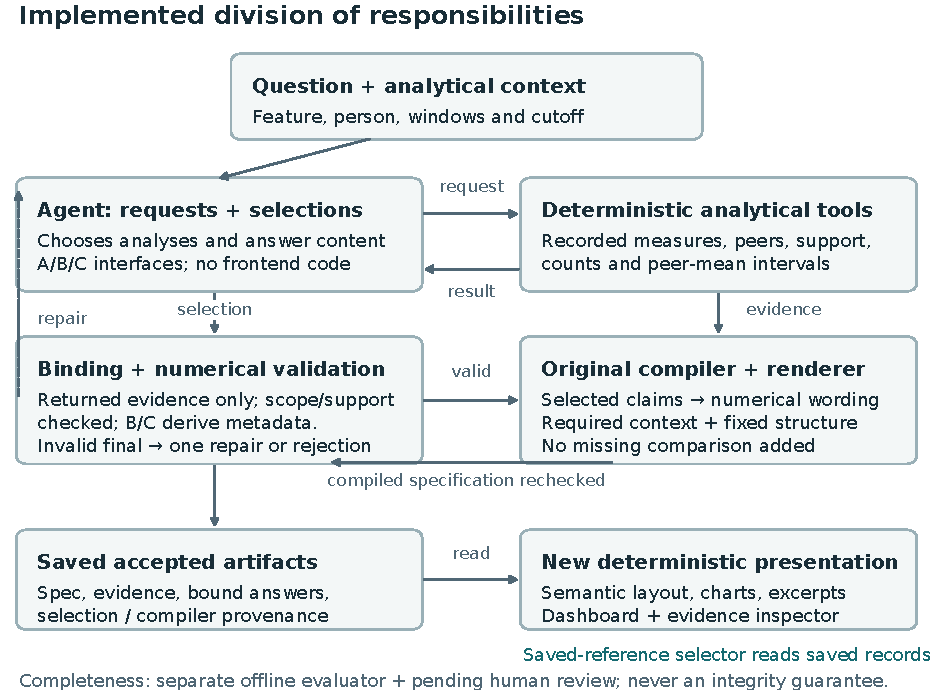
\includegraphics[width=\textwidth]{figures/architecture.pdf}
\caption{Implemented responsibilities. The agent chooses analytical requests and answer content; deterministic tools calculate values. Binding and validation can reject a final answer or permit one repair. The original compiler supplies tagged structure and context, without adding a missing comparison claim. A later presentation layer reads saved accepted artifacts; its reference selector does not call the model. Numerical validity and question completeness are checked separately.}
\label{fig:architecture}
\end{figure*}

\subsection{Evidence, Binding and Validation}
Evidence records retain features, units, focal/reference windows, counts, estimates, support, observation/assessment states, uncertainty, source/configuration hashes, seeds, and execution metadata. Model context omits raw rows; full evidence remains available for inspection.

A peer answer has analytical identity
\begin{equation}
I_{\mathrm{peer}}=(i,o,t,f,W_f,g,W_g),
\end{equation}
where $i$ is the focal person, $o$ the offering, $t$ the cutoff, $f$ the feature, $W_f$ the focal window, $g$ the reference definition, and $W_g$ its window. A personal-history identity instead contains
\begin{equation}
I_{\mathrm{personal}}=(i,o,t,f,W_b,W_r).
\end{equation}
Personal meaning excludes irrelevant peer definitions. Exact readable handles are generated only from returned evidence, not hidden desired answers.

Unknown, ambiguous, or altered identities fail without substitution or added analysis. Personal summaries repeated across evidence records are equivalent only if person, feature, units, cutoff, windows, means, counts, change, and support agree exactly. Resolution chooses a stable returned identifier and retains aliases; it creates no peer answer.

Validation reconstructs expectations from the trusted development bundle, checking summaries, trajectories, counts, interval endpoints, units, references, windows, eligibility, and cutoff. A recomputed content hash cannot legitimize mutated values. Numerical text binds to validated fields; unsupported scope or identifiers fail despite valid JSON. This establishes fidelity to the implementation, not scientific adequacy or question completeness.

\subsection{Compiler and Provenance}
The vocabulary comprises peer comparison, personal change, assessment status, observation status, and measurement limitation. Peer selections produce comparison claims/panels; personal selections produce personal claims/trajectories. Support rules yield descriptive or scoped-insufficiency wording. Unknown grades remain unavailable measurements.

The common contract supplies required trajectories, observation/assessment context, and qualifications, but no missing comparison or personal claim. Supplied timelines or grade limitations can nevertheless answer a requested item. Provenance separates selections, resolutions, metadata, and compiler additions. Every number is calculated and inserted deterministically: ``model-selected'' means chosen content, never model-authored arithmetic.

\subsection{Adaptive Presentation of Saved Answers}
Publication views postdate the experiment and reorganize saved content without new evidence, changed windows, repaired omissions, or rescoring. Layout follows semantics, not case identifiers. Exact personal duplicates may collapse with checked equivalence and preserved multiplicity; distinct peer claims remain in expanded views. Completeness is judged from full original dashboards, not publication crops.

Figure~\ref{fig:adaptation} contrasts a personal trajectory with a selected peer comparison against a view of recorded zeros, ineligibility, and unavailable quantities. The original compiler supplied the latter's observation timeline and grade context; presentation did not discover them. Assessment views instead emphasize observed-week submission measures and dated states. All views provide an expandable evidence inspector and source-method information.

\begin{figure*}[!t]
\centering
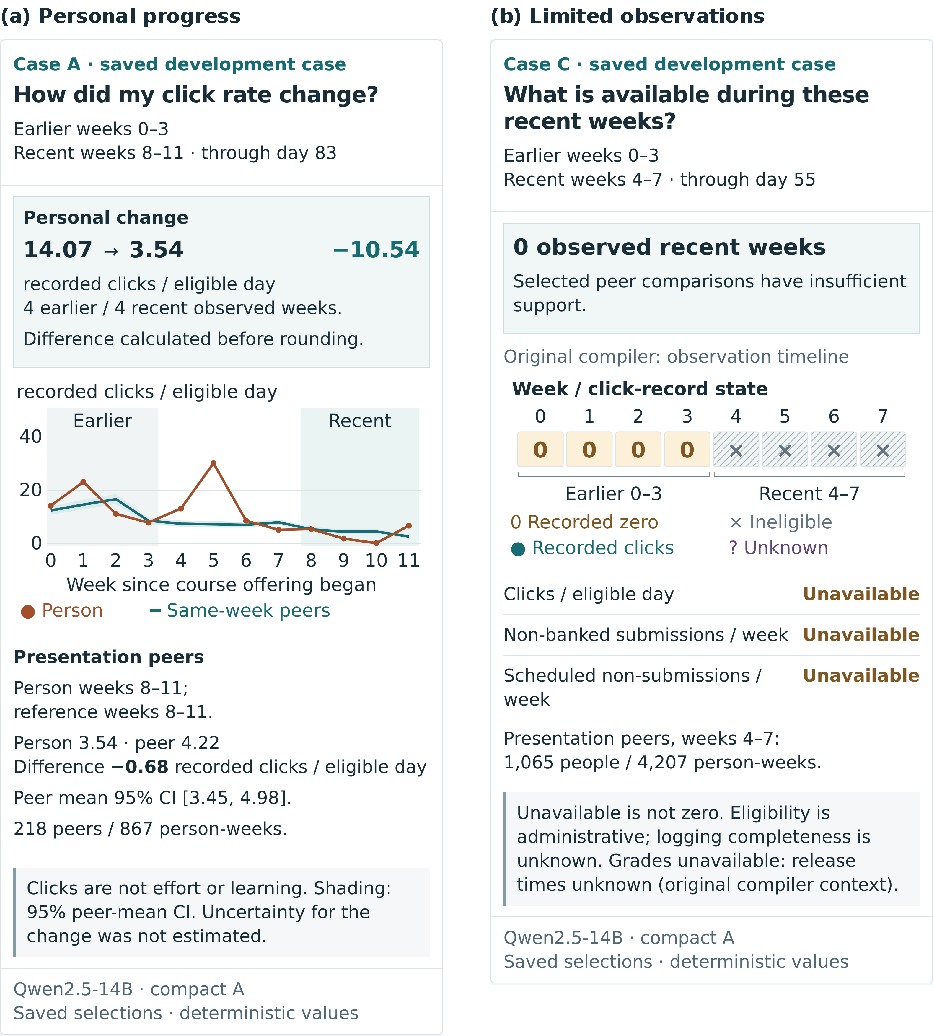
\includegraphics[width=\textwidth]{figures/adaptation.pdf}
\caption{New renderings of saved development answers from compact condition A. (a) Case 01: selected personal change and recent-peer context. The unrounded means produce the displayed change; the shaded band is a pointwise 95\% peer-mean bootstrap interval, not uncertainty for personal change. (b) Case 09: recorded zero activity is distinct from ineligibility and unavailable recent quantities. This answer was accepted after one historical repair; its original compiler supplied the observation timeline and grade-availability context. Anonymous display aliases differ from experimental condition labels. Deterministic presentation adaptation establishes neither improved accuracy nor usability.}
\label{fig:adaptation}
\end{figure*}

Reference comparisons use aligned scales and explicit focal and reference windows. In Figure~\ref{fig:reference}, a working selector switches between two comparisons already selected by the same agent. It updates the highlighted result, counts, labels, chart, and evidence link together. The focal measurement stays fixed while the reference period changes. This is viewing saved analysis, not a new investigation or statistical recomputation. Full and excerpted views retain the distinction between unavailability and zero, and peer-mean intervals are not repurposed as uncertainty for a contrast.
\section{\uppercase{Experiment}}
\label{sec:experiment}
\noindent Four conditions answer the same questions for 24 new development people, four per known family. Earlier development established the backend, generic policy, compiler, and evaluator; its focal people are excluded. Those earlier results motivate the ablation but are not pooled as confirmation evidence.\draftassist

\subsection{Cases and Shared Information}
Six families cover personal change with peers; comparisons across named references; observation availability; separate personal/recent-peer insufficiency; submission and scheduled non-submission means with assessment/grade context; and alternate earlier/recent windows. Reference questions do not automatically require personal change or a changed conclusion.

The frozen profiles use earlier/recent week pairs 0--3/8--11 at day~83, 0--3/4--7 at day~55, 0--1/2--3 at day~27, 0--3/10--11 at day~83, and 2--5/6--9 at day~69. Each question names the requested measure, windows, and cutoff. Candidate selection uses administrative eligibility and prior-attempt status where relevant. In particular, the insufficient-support family requires fewer than two recent eligible weeks and at least one earlier eligible week. It is not selected by searching for model failures or extreme activity.

Each structural slot selects the unused eligible person minimizing SHA256(seed, case, person), with seed \texttt{stage6-structural-v1-20260918}. All 57 previous and 24 new focal people are excluded from the shared reference pool across registrations. All cases are real observations. Separate row-loop calculations checked 52 fact records; this is an independent calculation path, not human review.

Conditions share public questions, family labels, definitions, references, windows, and interpretation rules. Hidden facts serve scoring and offline diagnosis only. Tasks, prompts, code, schemas, sources, settings, scoring, and order were frozen before inference, without post-freeze tuning or reruns until success.

\subsection{Conditions and Ablation}
\textbf{Enumeration} applies rules to the public task/reference registry, enumerating admissible references for relevant features and adding assessment measures where required. It shares the backend, validator, renderer, and six-call ceiling. Routing by public family makes it a strong registry baseline, not an unrestricted language interpreter.

\textbf{A: compact} selects answer kinds and returned identifiers, with model-authored support and scoped conclusion; its existing compiler builds the layout. \textbf{B: derived metadata} retains kind/identifier selection but derives support/scope, uses a neutral heading, and adds a mechanical catalogue of returned answers. B versus A tests this package, not metadata deletion alone.

\textbf{C: explicit binding} selects exact handles using B's metadata behavior and identical catalogue. C versus B tests identity representation under equivalent information; C versus A tests the entire intervention. All agents share the generic policy, and none receives hidden requirements or automatic missing comparisons. Valid irrelevant selections remain possible.

\subsection{Model, Budgets and Ordering}
All agents use Qwen2.5-14B-Instruct \cite{qwenReport,qwenCheckpoint}, pinned to revision \texttt{cf98f3b3bbb457ad9e2bb}\allowbreak\texttt{7baf9a0125b6b88caa8}. The Transformers 4.55.2 backend uses the checkpoint's tokenizer and chat template, Torch 2.8.0+cu128, CUDA~12.8, BF16, and scaled dot-product attention. All parameters, inputs, and generated outputs resided on one RTX~6000 Ada GPU; there was no quantization or CPU offload. Process residency, per-generation device timing, and CUDA profiling substantiate GPU execution, rather than a CUDA-availability check alone.

Greedy decoding permits 16,000 input and 1,500 output tokens. Episodes allow six analytical calls, four generations, and one final repair using integrity errors and existing evidence, never completeness feedback. Invalid actions, failed specifications, and repairs are retained. There is no constrained decoding, training, or fallback success.

Enumeration ran on the same host's CPU. Six A/B/C permutations repeat four times, balancing positions and pair order. One model load served 72 agent episodes; all 96 method/case slots were attempted once. Timing is descriptive, and greedy decoding does not measure stochastic repeatability.

\subsection{Endpoints and Their Limits}
An \emph{accepted output} passes schema, support/scope, evidence, numerical, and rendering checks. First-final validity excludes later repairs but allows prior tool errors. \emph{Complete visible answers} require acceptance and every requested answer under the frozen evaluator. Required context is separately tracked and present for all visibly complete cases; optional panels earn no automatic answer credit.

\emph{Completeness through method selections} uses the same predicates after projecting out compiler-only claims, panels, and boilerplate. Selections are deterministic for enumeration and model choices for agents; neither means model-calculated numbers. Insufficiency must match the feature, window, and comparison, without excusing other omissions.

Paired complete valid visible answers are primary; selected completeness, validity, costs, and failures are secondary. All slots remain in denominators. An offline oracle-assisted retrieved-evidence upper bound uses hidden requirements only for diagnosis. No significance tests are added. The prespecified gate was 22/24 visibly complete, zero accepted unsupported quantities, and both answers on all four insufficiency cases; it is not a conference acceptance criterion.
\section{\uppercase{Results}}
\label{sec:results}
\noindent All 96 method/case slots were attempted. Table~\ref{tab:outcomes} and Figure~\ref{fig:results} are generated directly from frozen machine-readable reports. Enumeration answered \EnumVisible/24 questions completely through its own selections. A produced \AVisible/24 complete visible answers, B \BVisible/24, and C \CVisible/24. Model-selected completeness was \ASelected/24, \BSelected/24, and \CSelected/24, respectively. These frozen values include the scoring caveat discussed below; they are not newly adjudicated accuracy estimates.\draftassist

\begin{table*}[!t]
\caption{Frozen outcomes. Every main endpoint retains all 24 cases per condition. ``Selected complete'' excludes compiler-supplied requested answers; enumeration's selections are deterministic. ``Both insuff.'' uses the four cases requesting separate personal and peer insufficiency answers. B's completeness has the answer-form caveat in Section~\ref{sec:caveat}.}
\label{tab:outcomes}
\centering\setlength{\tabcolsep}{4pt}
% BEGIN GENERATED: outcomes
%% Generated from frozen reports; do not edit.
\begin{tabular}{lrrrrr}
\hline
Condition & First valid & Accepted & Visible complete & Selected complete & Both insuff. answers \\
\hline
Enumeration & 24/24 & 24/24 & 24/24 & 24/24 & 4/4 \\
A: compact & 21/24 & 22/24 & 21/24 & 18/24 & 3/4 \\
B: derived metadata & 22/24 & 24/24 & 15/24 & 14/24 & 2/4 \\
C: explicit binding & 21/24 & 21/24 & 15/24 & 11/24 & 1/4 \\
\hline
\end{tabular}
% END GENERATED: outcomes
\space % Preserve the trailing space from the original table input.
\end{table*}

\begin{figure*}[!t]
\centering
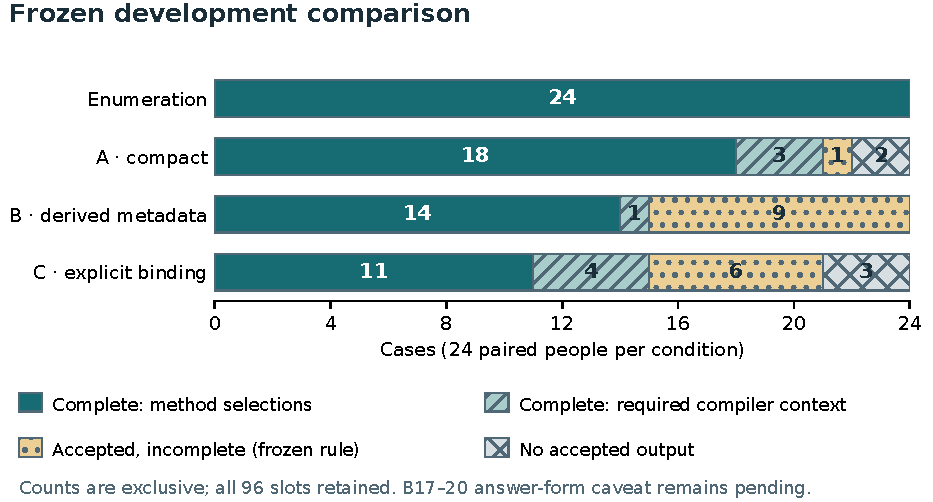
\includegraphics[width=\textwidth]{figures/results.pdf}
\caption{Frozen development comparison on 24 paired people. Categories are mutually exclusive: complete through method selections; otherwise complete with required compiler context; otherwise accepted but incomplete; or no accepted output. All numbers, even in model-selected answers, come from deterministic tools. B17--20 visibly contain requested recent means in personal-change claims that the frozen focal predicate does not credit. These four cases remain in the incomplete category pending human adjudication. No score is revised here.}
\label{fig:results}
\end{figure*}

\subsection{Validity, Completeness and Attribution}
B achieved 24 accepted outputs, compared with 22 for A and 21 for C, but its frozen visible completeness remained lower than A's. Successful final repairs were one of three for A, two of two for B, and zero of three for C. Rejections remained in the denominator; there were no infrastructure-blocked episodes or deterministic fallbacks. No agent met the combined engineering target.

Compiler-supplied requested context completed three additional A cases, one B case, and four C cases. Its 32, 37, and 37 added panels contained no added comparison or personal-change claim. Panel count is not a quality score. Supplied grade limitations, for example, can answer a request without model selection.

In paired outcomes (Table~\ref{tab:paired}), C loses six visible complete cases relative to A and has no net gain over B: three improve and three regress. Selected completeness is seven below A and three below B. These frozen results do not support a binding benefit; disputed B judgments qualify the equality with C.

\begin{table}[t]
\caption{Paired visible completeness on the same 24 people. ``Right only'' and ``Left only'' refer to the named contrast. Counts are descriptive, with no significance test.}
\label{tab:paired}
\centering\setlength{\tabcolsep}{3pt}
% BEGIN GENERATED: paired
%% Generated from frozen reports; do not edit.
\begin{tabular}{lrrrr}
\hline
Right $-$ left & Both & Right only & Left only & Neither \\
\hline
C $-$ A & 14 & 1 & 7 & 2 \\
C $-$ B & 12 & 3 & 3 & 6 \\
B $-$ A & 14 & 1 & 7 & 2 \\
\hline
\end{tabular}
% END GENERATED: paired
\space % Preserve the trailing space from the original table input.
\end{table}

\subsection{Evidence Retrieval and Failure Mechanisms}
The offline diagnostic found sufficient returned evidence for all 24 questions in both A and B, and 21 in C. In case~15, A nevertheless selected peer comparisons for weeks~0--3 when asked about weeks~10--11. Returned recent evidence supported a separate personal-insufficiency answer, but its peer answer was omitted (Figure~\ref{fig:failure}). Correct earlier-window binding does not establish relevance.

C12 selected an earlier result for a requested recent mean. Invalid C18--20 analysis batches returned no evidence; final/repair handles remained unresolved. No catalogue had been returned, so its contents alone cannot explain those failures. A09 repaired peer selections paired with personal conclusion scope; A12 did not. A22 retained invalid scope; B23 repaired a panel-limit error. These are trace observations, not established cognitive causes.

All 168 comparison generations reached end-of-sequence, with at most 491 output tokens: failures were not output-limit truncation. Source checks detected no accepted unsupported quantitative answer among 91 accepted dashboards. This bounded result establishes agreement with checked fields/support rules, not universal semantic correctness or completeness.

\subsection{Unresolved Answer-Equivalence Caveat}
\label{sec:caveat}
B17--20 display both requested recent assessment means within supported personal-change claims. The frozen focal-item predicate recognizes a comparison panel or a supported comparison claim, but does not inspect a personal-change claim for that mean. It therefore classifies eight requested items as retrieved but omitted even though their feature, units, recent window, and values appear on the page. This is an evaluation representation limitation, not a numerical failure. B remains 15/24 visible complete and 14/24 selected complete in every reported table and figure; no disputed case receives new credit.

C21/C23 display earlier and recent means in peer claims without an explicit personal-change answer; equivalence is a separate unresolved question. Unavailable forms and scoped insufficiency also require review. All 96 original slots, including rejections, are prepared for two reviewers and adjudication, but no ratings exist. Automated inspection is not independent human review, and frozen completeness is not a settled measurement construct.

\begin{figure*}[!t]
\centering
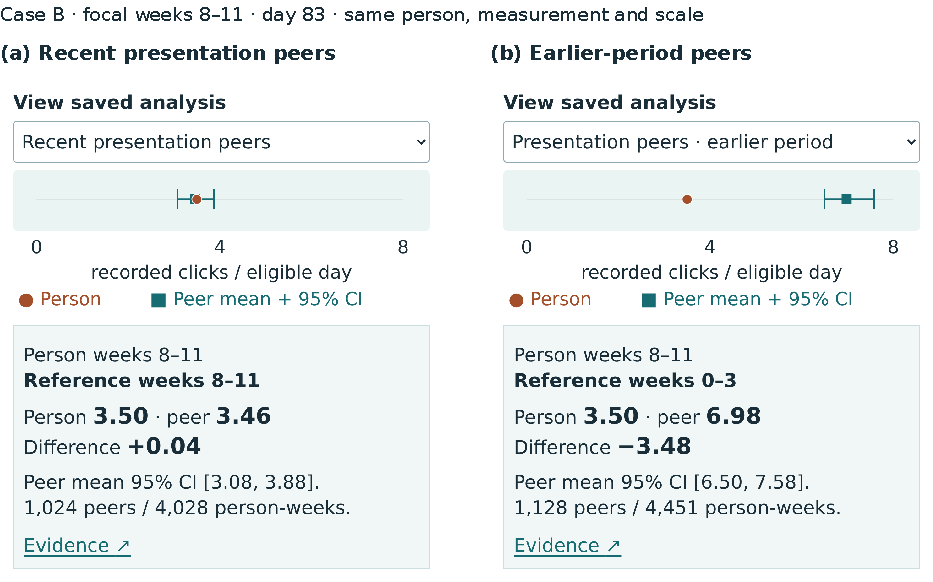
\includegraphics[width=\textwidth]{figures/reference_switch.pdf}
\caption{A saved reference-period change in condition A, case~05. Both comparisons were model-selected. Browser excerpts show the selector reading validated records, not recomputing statistics. The person, focal weeks~8--11, units, and scale stay fixed; the reference changes from weeks~8--11 to weeks~0--3. Eligible membership differs (1,024 versus 1,128 people). Whiskers are 95\% bootstrap intervals for peer means, not for contrasts. The later presentation layer supplies the layout. Earlier peers are not necessarily fairer or causally adjusted.}
\label{fig:reference}
\end{figure*}

\subsection{Recorded Cost}
Table~\ref{tab:costs} retains failures and repairs. Enumeration used more calls but far less episode time and no inference. C used more generations and equivalent repeated analyses than either control without higher completeness. This supports enumeration's operational economy within the registry.

\begin{table*}[!t]
\caption{Recorded comparison costs summed over 24 cases per condition. Episode time includes analytical and rendering work; shared model loading/profiling is separate. $^{a}$Exact/equivalent repeated requests use the frozen signatures; equivalent requests share feature, group and window meaning. Input/output token totals count repeated context, failures, and repairs.}
\label{tab:costs}
\centering\setlength{\tabcolsep}{3pt}
% BEGIN GENERATED: costs
%% Generated from frozen reports; do not edit.
\begin{tabular}{lrrrrrr}
\hline
Condition & Tools & Repeated$^{a}$ & Generations & Input / output tokens & Episode s & Median s \\
\hline
Enumeration & 84 & 0 / 0 & 0 & 0 / 0 & 35.40 & 1.18 \\
A: compact & 76 & 0 / 5 & 52 & 178,794 / 10,274 & 484.64 & 17.07 \\
B: derived metadata & 79 & 0 / 8 & 53 & 238,675 / 10,012 & 504.21 & 16.87 \\
C: explicit binding & 82 & 4 / 12 & 63 & 262,031 / 10,695 & 536.32 & 21.19 \\
\hline
\end{tabular}
% END GENERATED: costs
\space % Preserve the trailing space from the original table input.
\end{table*}

Including setup/construction, 185 generations used 1,719.02~s of model-process time (28.65~min), including loading/cleanup: 153.02~s construction and 1,566.00~s comparison. Shared comparison loading/profiling took 37.55/1.65~s. Peak allocated/reserved memory was 30.78/35.23~GiB; maximum input was 10,888 tokens. Process time, episode latency, and implementation wall time differ and do not establish billing time. Manuscript preparation ran no experimental inference.
\section{\uppercase{Discussion and Limitations}}
\label{sec:discussion}
\noindent Correct computation and exact binding cannot ensure selection of the requested result. Case~15 contains personal insufficiency but substitutes valid earlier comparisons for the requested recent-peer answer. Silently inserting that answer would hide the selection failure being studied.\draftassist

\begin{figure*}[!t]
\centering
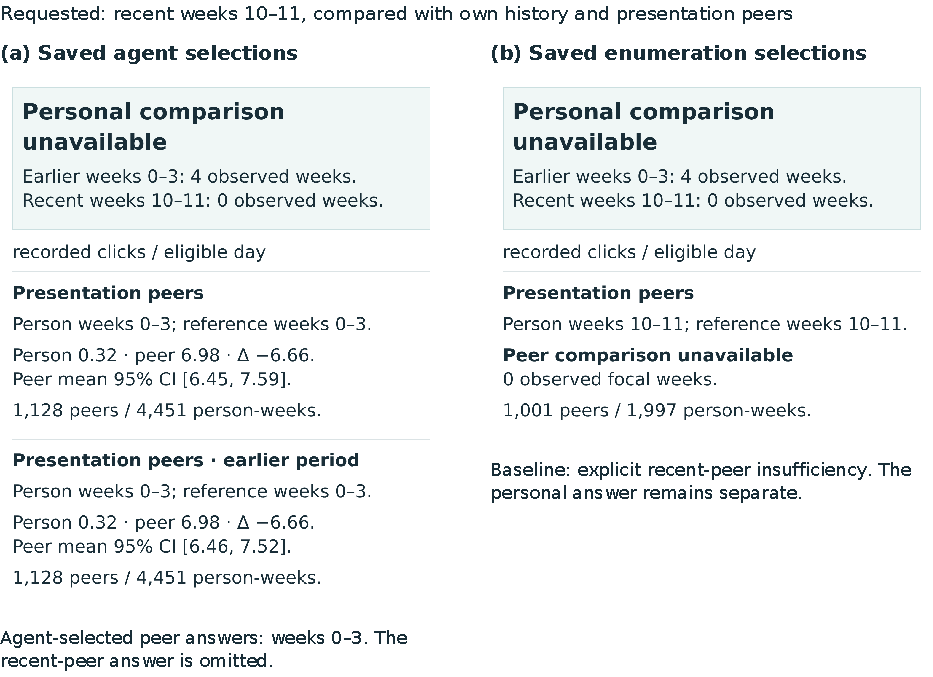
\includegraphics[width=\textwidth]{figures/failure.pdf}
\caption{Correct source-bound values with an incomplete answer, case~15. The request concerns weeks~10--11 and separately asks about own history and peers. (a) A selects earlier peer answers for weeks~0--3 and retains a personal-insufficiency answer. (b) Enumeration explicitly supplies the recent-peer insufficiency answer, also retaining personal insufficiency. Reviewer annotations outside the faithful excerpts identify the mismatch; the agent's missing answer is not inserted. Full original dashboards, not these cropped views, determine the frozen judgment. Intervals describe peer means; unavailable is not zero.}
\label{fig:failure}
\end{figure*}

\subsection{What the Ablation Establishes}
Explicit identity yielded no frozen visible gain over B and lower completeness than A. B's higher acceptance did not establish better coverage, and its catalogue prevents attributing effects solely to metadata derivation. Traces expose selection relevance, malformed requests, and incomplete scope coverage without isolating their causal contributions.

Counting all visible context as agent reasoning would overstate model responsibility; treating every frozen omission as literal absence would misdescribe B17--20. Provenance and equivalent-answer adjudication are both needed. Additional panels alone do not establish a better answer.

Enumeration remains the operational baseline. Its public task-family label and small registry make exhaustive rules feasible; success does not establish unrestricted language understanding. Agent benefits for ambiguous requests, larger registries, or other domains remain untested. Neither a per-case best-condition mixture nor further indefinite prompt tuning is justified.

\subsection{Presentation as an Inspectable System Behavior}
Figure~\ref{fig:reference} holds the focal rate at 3.50 clicks per eligible day while switching recent/earlier peer means of 3.46/6.98. Saved differences are +0.04/$-3.48$, calculated before rounding. Changed period and membership remain visible. This shows reference dependence of a description, not causation or reference superiority.

The assessment view foregrounds measures and events. In A17, recent weeks~8--11 have 0.25 non-banked submissions per observed week and zero scheduled non-submissions, while a day-55 snapshot records no submission for the day-54 assessment. Their temporal scopes differ; later submissions do not rewrite earlier snapshots. Grades and banking approval remain unavailable, not achievement ratings. This is implemented adaptation, not measured usability or accuracy improvement.

\subsection{Threats to Interpretation}
There are 24 development people from two offerings, not 96 independent observations. Families and wording conventions were known. One checkpoint, greedy episode, and environment do not establish robustness across models, paraphrases, runs, or deployments. Reserved people remain unevaluated; earlier development is not independent confirmation.

The rubric needs adjudication against question meaning. Numerical agreement cannot settle reference appropriateness, support thresholds, or equivalent answers. Independent forms for all 96 slots remain blank; human review and usability evaluation are pending.

Repeated rows, unknown logging and grade timing, eligibility, changing peers, and unequal histories limit measurement interpretation. Bootstrap intervals do not quantify measurement error, causality, or individual risk. No prediction, anomaly detection, or assessment of ability is validated. Presentation does not remedy these limits.

Any adjudicated reanalysis must be separately versioned as post hoc. Stronger reliability claims need a fixed system/scorer, person-level sampling, enumeration controls, and prespecified outcomes before reserved-data evaluation. The internal gate is not a conference acceptance requirement; its failure limits operational claims, rather than automatically invalidating a negative development study.
\section{\uppercase{Conclusion}}
\label{sec:conclusion}
\noindent The implemented pipeline separates model selection, deterministic calculation, evidence binding, compiler context, and adaptive presentation. In 24 development cases, explicit identity did not improve frozen completeness; enumeration remained complete and cheaper. Valid source-bound numbers could accompany wrong-window answers or omissions, while compiler context could supply an unselected answer.\draftassist

The findings support separate responsibility and coverage accounting, not general claims about agents or usability. Equivalent-answer and measurement judgments require review before any fixed validation study. This is a bounded development analysis of completeness and its failure modes.
\section{\uppercase{AI Assistance Disclosure}}
\label{sec:disclosure}
\noindent OpenAI Codex \cite{openaiCodex} assisted all sections, the abstract, captions, bibliography, implementation, and figure/verification code, including substantive drafting and source tracing. This differs from the experimental Qwen checkpoint; drafting ran no experimental generations. Figures depict saved data or programmatic diagrams. Assisted checks are not independent human review. Author verification, adjudication, and disclosure placement remain pending. No AI system is an author.
\bibliographystyle{apalike}
\bibliography{references}
\end{document}
